% power-semiring.tex — publication-grade figure of lling-llang's η-power semiring
% Sₙ = (ℝ₊∪{+∞}, ⊕_η, ×, 0, 1) with ⊕_η x y = (x^{1/η}+y^{1/η})^η, and the
% η-controlled interpolation max ← probability → min, plus the Ψ_η isomorphism.
% Native ⊕/⊗/0̄/1̄ typography. Palette: docs/diagrams/README.md.
% Compile: lualatex --output-format=dvi power-semiring.tex ; dvisvgm --no-fonts power-semiring.dvi
\documentclass[dvisvgm,border=6pt]{standalone}
\usepackage{fontspec}
\usepackage{amsmath,amssymb}
\usepackage{tikz}
\usetikzlibrary{positioning,fit,backgrounds,arrows.meta}

% palette (docs/diagrams/README.md)
\definecolor{foundation}{HTML}{BBDEFB}\definecolor{foundationB}{HTML}{1565C0}
\definecolor{algorithms}{HTML}{C8E6C9}\definecolor{algorithmsB}{HTML}{2E7D32}
\definecolor{speech}{HTML}{FFE0B2}\definecolor{speechB}{HTML}{E65100}
\definecolor{nlp}{HTML}{FFF59D}\definecolor{nlpB}{HTML}{F9A825}
\definecolor{ink}{HTML}{102027}\definecolor{edge}{HTML}{607D8B}

\begin{document}
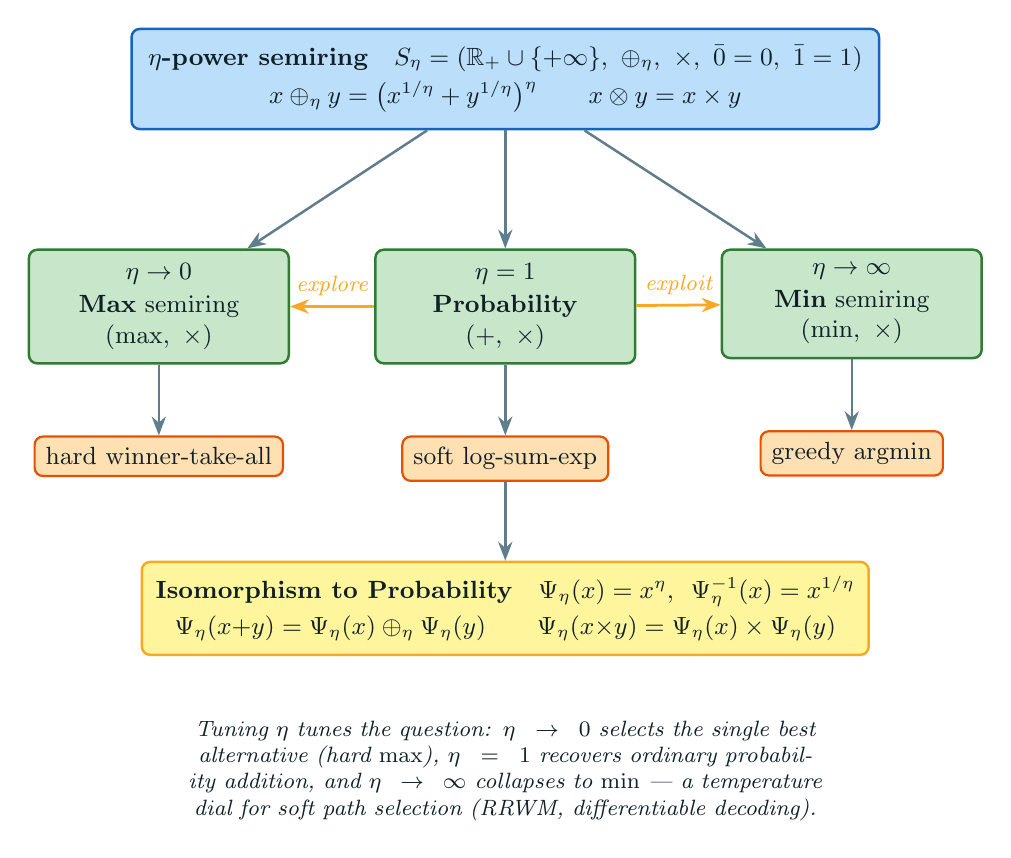
\begin{tikzpicture}[
    every node/.style={font=\small, text=ink},
    sig/.style={draw=foundationB, fill=foundation, rounded corners=3pt, align=center,
                inner sep=6pt, line width=0.9pt},
    lim/.style={draw=algorithmsB, fill=algorithms, rounded corners=3pt, align=center,
                inner sep=5pt, line width=0.9pt, minimum width=33mm},
    prop/.style={draw=speechB, fill=speech, rounded corners=3pt, align=center,
                 inner sep=4pt, line width=0.8pt},
    iso/.style={draw=nlpB, fill=nlp, rounded corners=3pt, align=center,
                inner sep=5pt, line width=0.9pt},
    rel/.style={-{Stealth[length=2.4mm]}, draw=edge, line width=0.9pt},
    arr/.style={-{Stealth[length=2.4mm]}, draw=nlpB, line width=1.0pt},
  ]

  % the signature, at the top
  \node[sig] (sig) {\textbf{$\eta$-power semiring}\quad
        $S_\eta=(\mathbb{R}_+\cup\{+\infty\},\ \oplus_\eta,\ \times,\ \bar 0=0,\ \bar 1=1)$\\[3pt]
        $x \oplus_\eta y = \bigl(x^{1/\eta}+y^{1/\eta}\bigr)^{\eta}
          \qquad x \otimes y = x\times y$};

  % the three limiting regimes
  \node[lim, below=15mm of sig, xshift=-44mm] (max)
        {$\eta \to 0$\\[1pt]\textbf{Max} semiring\\ $(\max,\ \times)$};
  \node[lim, below=15mm of sig]               (prob)
        {$\eta = 1$\\[1pt]\textbf{Probability}\\ $(+,\ \times)$};
  \node[lim, below=15mm of sig, xshift=44mm]  (min)
        {$\eta \to \infty$\\[1pt]\textbf{Min} semiring\\ $(\min,\ \times)$};

  \draw[rel] (sig) -- (max);
  \draw[rel] (sig) -- (prob);
  \draw[rel] (sig) -- (min);

  % the exploration ↔ exploitation axis between the regimes
  \draw[arr] (prob) -- (max) node[midway, above, font=\footnotesize\itshape, text=nlpB]{explore};
  \draw[arr] (prob) -- (min) node[midway, above, font=\footnotesize\itshape, text=nlpB]{exploit};

  % property tags under each regime
  \node[prop, below=9mm of max]  (maxp)  {hard winner-take-all};
  \node[prop, below=9mm of prob] (probp) {soft log-sum-exp};
  \node[prop, below=9mm of min]  (minp)  {greedy argmin};
  \draw[rel] (max)  -- (maxp);
  \draw[rel] (prob) -- (probp);
  \draw[rel] (min)  -- (minp);

  % the isomorphism box
  \node[iso, below=10mm of probp] (isom)
        {\textbf{Isomorphism to Probability}\quad
         $\Psi_\eta(x)=x^{\eta}$,\ \ $\Psi_\eta^{-1}(x)=x^{1/\eta}$\\[2pt]
         $\Psi_\eta(x{+}y)=\Psi_\eta(x)\oplus_\eta\Psi_\eta(y)
          \qquad \Psi_\eta(x{\times}y)=\Psi_\eta(x)\times\Psi_\eta(y)$};
  \draw[rel] (probp) -- (isom);

  % caption
  \node[below=7mm of isom, text width=104mm, align=center, font=\footnotesize\itshape]
        {Tuning $\eta$ tunes the question: $\eta\to0$ selects the single best alternative
         (hard $\max$), $\eta=1$ recovers ordinary probability addition, and
         $\eta\to\infty$ collapses to $\min$ — a temperature dial for soft path selection
         (RRWM, differentiable decoding).};
\end{tikzpicture}
\end{document}
